\documentclass[12pt]{article}

\usepackage[hmargin=2.5cm, vmargin={3cm,3cm}, a4paper]{geometry}
\usepackage{amsmath,amssymb,amsthm,mathrsfs}
\usepackage{epsfig,epsf,subfigure,graphicx,graphics}
\usepackage{url,enumerate}
\usepackage{physics,dsfont}
\graphicspath{{fig/}}
\usepackage{fancyhdr}
\setlength{\headheight}{12pt}
\pagestyle{fancyplain}

\numberwithin{equation}{section}
\newtheorem{theorem}{Theorem}

% definitions/operators
\DeclareMathOperator*{\argmax}{arg\,max\;}
\DeclareMathOperator*{\argmin}{arg\,min\;}
\newcommand{\eqtext}[1]{\ensuremath{\stackrel{#1}{=}}} % equal sign with some text over it
\renewcommand{\thesubsection}{\thesection.\alph{subsection}} % to use letters for subsections
\newcommand\independent{\protect\mathpalette{\protect\independenT}{\perp}} % see next one
\def\independenT#1#2{\mathrel{\rlap{$#1#2$}\mkern2mu{#1#2}}} % to have independet symbol

\rhead{}
\lhead{}
\chead{{\it Network Information Theory}}
\lfoot{}
\cfoot{\thepage}
\rfoot{}
\title{Solution of Homework \#1}
\author{Mattia Lecci, Federico Mason}
\begin{document}
\maketitle
\thispagestyle{fancyplain}
\flushleft


%% execises
\section{Problem 3.2}

\begin{figure}[h]
	\centering
	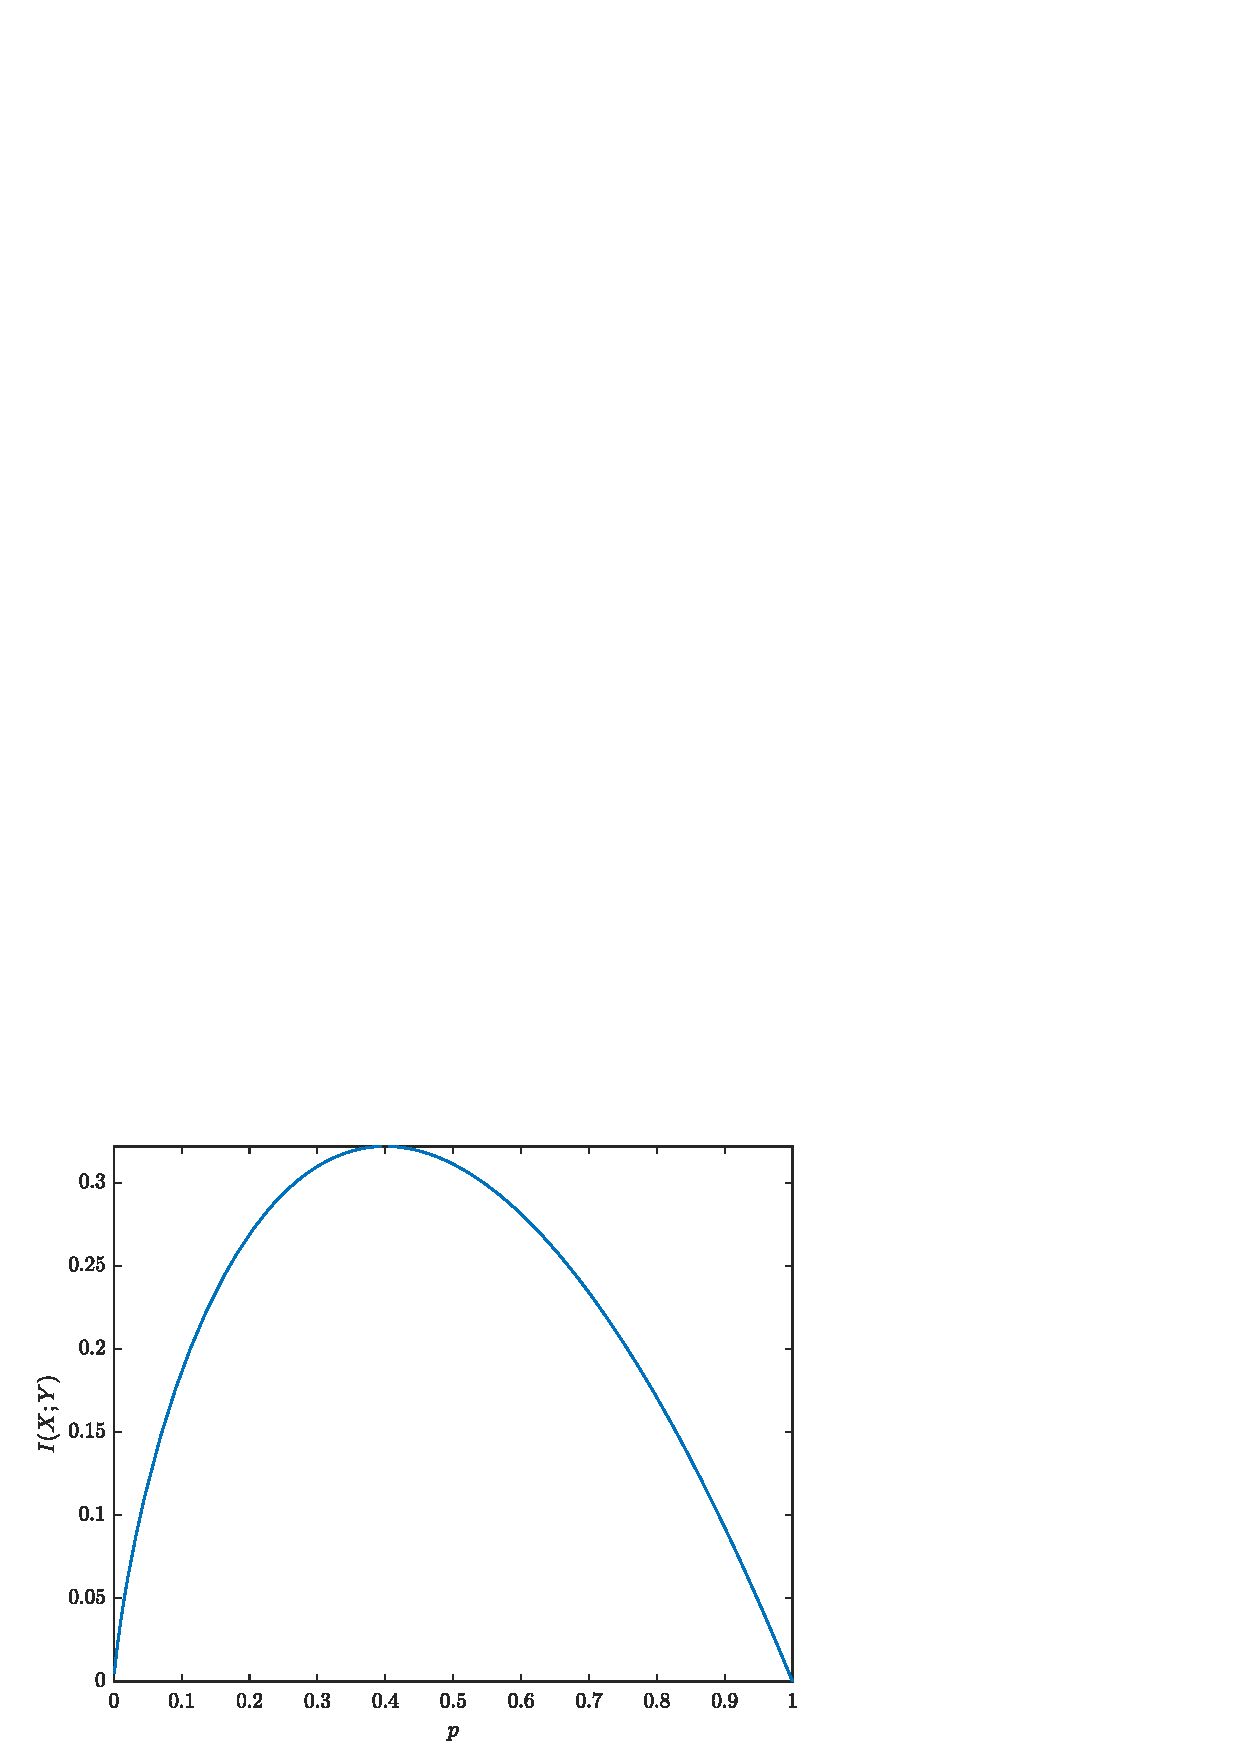
\includegraphics[width=0.7\linewidth]{img/func_info_ex1}
	\caption{Mutual information as a function of $p \triangleq p_X(1)$}
	\label{fig:funcinfoex1}
\end{figure}

\mysection{4.12}{Problem 4.12}

Since we are interested in creating lists of length $\LL_2 \leq 2^{nL_2}$, we could think of dividing the original set of messages into equal length lists and sending the index of the list instead. In other words, we could think of dividing the $|\M_2| = 2^{nR_2}$ into $|\K_2| = 2^{nR_2}/2^{nL_2} = 2^{n(R_2-L_2)}$ lists $\qty{ \LL_1, \dots,\LL_{2^{n(R_2-L_1)}} }$ of $2^{nL_2}$ messages each (assuming $R_2$ and $L_2$ integers just for simplicity). Thus, we can create a function $K: \M_2 \rightarrow \K_2$ that returns the index of the list in which a specific message is contained. Just for convenience we force $K(1)=1$. Furthermore, we will treat this list number similarly to how we treat normal messages, thus encoding it using an alphabet $\Z_2$ through the function $Z_2^n(k_2) = Z_2^n(K_2(m_2))$. At this point we can easily treat the word $Z_2^n$ like we would treat $X_1^n$ or $X_2^n$.

Like a normal MAC, the transmitters send the couple $(X_1^n(M_1),Z_2^n(K_2))$ (where $K_2 = K_2(M_2)$) and the receiver decodes $(\hat{M}_1,\hat{K}_2)$.

Let's fix $p(x_1,x_2) = p(x_1)p(x_2)$. Note that averaging over all the possible random codebooks we obtain and using our notation, we obtain
%
\begin{equation}
\Pen = \Pr(M_1 \neq \hat{M}_1 \cup M_2 \notin \LL_{\hat{K}_2} | M_1=M_2=1 ) \triangleq \Pr(\E | M_1=M_2=1)
\end{equation}

The error event can be decomposed into
%
\begin{align}
\begin{split}
\E =& \qty{ \qty(X_1^n(1),Z_2^n(1),Y^n) \notin \typicalitySet }\\
\cup& \{ \exists m_1\neq 1: (X_1^n(m_1),Z_2^n(1),Y^n) \in \typicalitySet \}\\
\cup& \{ \exists m_2\neq 1: (X_1^n(1),Z_2^n(m_2),Y^n) \in \typicalitySet \}\\
\cup& \{ \exists m_1,m_2\neq 1: (X_1^n(m_1),Z_2^n(m_2),Y^n) \in \typicalitySet \}\\
\triangleq& \E_1 \cup \E_2 \cup \E_3 \cup \E_4
\end{split}
\end{align}

As usual, we know from the \textit{Law of Large Numbers} that $\E_1 \xrightarrow{n \rightarrow \infty} 0$.

Considering $\E_2$, it's clear that $p(x_1^n,z_2^n,y^n) = p(x_1^n)p(z_2^n)p(y^n|z_2^n)$. Thus, $X_1^n(m1) \independent (\LL_1,Y^n)$, hence
%
\begin{eqnarray}
\Pr(\E_2) \rightarrow 0 & \text{if } R_1 < I(X_1;Z_2,Y) = I(X_1;Y|Z_2)
\end{eqnarray}
%
where the last equality holds from the independence.

Similarly we obtain
%
\begin{align}
\begin{split}
\Pr(\E_3) \rightarrow 0 \quad& \text{if } R_2-L_2 < I(Z_2;X_1,Y) = I(Z_2;Y|X_1)\\
\Pr(\E_4) \rightarrow 0 \quad& \text{if } R_1+R_2-L_2 < I(X_1,Z_2;Y)
\end{split}
\end{align}
%
where the $R_2-L_2$ terms come from the fact that $Z_2^n$ is a function of elements of $\K_2$ which has cardinality equal to $2^{n(R_2-L_2)}$.

Thus, considering all possible probability distributions as well as time sharing, we obtain that $\Pen \rightarrow 0$ if
%
\begin{equation}
(R_1,R_2) \in \conv{\bigcup_{p(x_1),p(z_2)}
\left\{
\begin{array}{rcl}
R_1 &<& I(X_1;Y|Z_2)\\
R_2 &<& I(Z_2;Y|X_1) + L_2\\
R_1+R_2 &<& I(X_1,Z_2;Y) + L_2
\end{array}
\right.
}
\end{equation}

%%%%%%%%%%%%%%%%%%%%%%%%%%%%%%%%%%%%%%%%%%%%%%%%%%%%%%%%%%%%%%%%%%%
%%%%%%%%%%%%%%%%%%%%%%%%%%%%%%%%%%%%%%%%%%%%%%%%%%%%%%%%%%%%%%%%%%%
%%%%%%%%%%%%%%%%%%%%%%%%%%%%%%%%%%%%%%%%%%%%%%%%%%%%%%%%%%%%%%%%%%%

To demonstrate the converse we need to modify once again Fano's inequality. We define $E = \indicator[\E]$, where $\indicator$ is the indicator function. Note that $\Pr(E=1) = \Pen$. After some simple manipulation (the same as last time) we obtain that
%
\begin{equation}
H(M_1,M_2|\hat{M}_1,\hat{K}_2) = \ldots \leq 1 + H(M_1,M_2|E,\hat{M}_1,\hat{K}_2)
\end{equation}

Then we can compute
%
\begin{align}
\begin{split}
H(M_1,M_2|E,\hat{M}_1,\hat{K}_2) =& \Pen H(M_1,M_2|E=1,\hat{M}_1,\hat{K}_2) + (1-\Pen) H(M_1,M_2|E=0,\hat{M}_1,\hat{K}_2)\\
\leq& \Pen \log_2 \qty(2^{nR_1}2^{nR_2}) + (1-\Pen) \log_2 \qty(2^{nL_2})\\
=& \Pen n(R_1+R_2-L_2) + nL_2
\end{split}
\end{align}

Joining everything back in the original equation we obtain
\begin{align}
\begin{split}
H(M_1,M_2|\hat{M}_1,\hat{K}_2) \leq& 1 + H(M_1,M_2|E,\hat{M}_1,\hat{K}_2)\\
\leq& 1 + nL_2 + n\Pen (R_1+R_2-L_2)\\
=& nL_2 + n \qty(\frac{1}{n} + \Pen (R_1+R_2-L_2))\\
=& n (L_2 + \varepsilon_n)
\end{split}
\end{align}
where $\varepsilon_n$ vanishes if $\Pen \rightarrow 0$.

Notice that from the conditional entropy properties and the data processing inequality ($(M_1,M_2)\rightarrow Y^n \rightarrow (\hat{M}_1,\hat{K}_2)$) we have:
%
\begin{equation}
H(M_2|Y^n,M_1) \leq H(M_1,M_2|Y^n) \leq H(M_1,M_2|\hat{M}_1,\hat{K}_2) \leq n(L_2 + \varepsilon_n)
\end{equation}

Thus,
%
\begin{align}
\begin{split}
nR_2 \leq& H(M_2) = H(M_2|M_1)\\
=& I(M_2;Y^n|M_1) + H(M_2|Y^n,M_1)\\
\leq& I(M_2;Y^n|M_1) + n(L_2 + \varepsilon_n)\\
\leq& \ldots\\
\leq& \sum_{i=1}^n I(X_{2i};Y_i|X_{1i}) + n(L_2 + \varepsilon_n)
\end{split}
\end{align}
\begin{eqnarray}
\begin{split}
\implies R_2 &\leq \frac{1}{n} \sum_{i=1}^n I(X_{2i};Y_i|X_{1i}) + L_2 + \varepsilon_n\\
&\leq I(X_2;Y|X_1,Q) + L_2 + \varepsilon_n
\end{split}
\end{eqnarray}
%
with the classical trick of the time-sharing variable.

In a similar way we can obtain
%
\begin{equation}
R_1 + R_2 \leq I(X_1,X_2;Y|Q) + L_2 + \varepsilon_n
\end{equation}

Lastly, we notice that also $M_1 \rightarrow Y^n \rightarrow \hat{M}_1$, yielding
%
\begin{equation}
H(M_1|Y^n,M_2) \leq H(M_1|Y^n) \leq H(M_1|\hat{M}_1) \leq n\varepsilon_{1,n}
\end{equation}
%
and with similar steps as before we obtain
%
\begin{equation}
R_1 \leq I(X_1;Y|X_2,Q) + \varepsilon_{1,n}
\end{equation}
%
where $\varepsilon_{1,n}$ depends on $\Pr(M_1 \neq \hat{M}_1|M_1=1) \triangleq P_{e1}^{(n)} \leq \Pen$

For all of these we need $\Pen \rightarrow 0$ so to obtain the following region:
%
\begin{equation}
\begin{cases}
R_1 &\leq I(X_1;Y|X_2,Q)\\
R_2 &\leq I(X_2;Y|X_1,Q) + L_2\\
R_1+R_2 &\leq I(X_1,X_2;Y|Q) + L_2
\end{cases}
\end{equation} %%%%%%%% fix!!
%\section{Problem 3.13}
\mysection{3.13}{Problem 3.13}

\numberwithin{equation}{subsection}

A Gaussian product channel $Y_j = g_j X_j + Z_j$, $j\in \{1,2\}$ with $g_1 < g_2$ and average power constraint $P$ is given. We want to know above what power $P^*$ we start to use both channels and what are the features of the \textit{energy-per-bit-rate function} $E_b(R)$.

\subsection{Optimal power allocation}

We notice that to achieve the maximum capacity from the channel we have to solve the following optimization problem
%
\begin{equation}\label{optproblem}
\begin{aligned}
&\max_{P_j} && \sum_{j=1}^2 \frac{1}{2} \cdot \log(1+g_j^2 \cdot P_j)\\
&\text{subject to}&& -P_j \leq 0 \quad j\in \{1,2\} \\
& 		   && \sum_{j=1}^2 P_j - P = 0
\end{aligned}
\end{equation}

%In order to solve \eqref{optproblem} we build the following equation
%%
%\begin{equation}
%	\nabla_{P_j}\Big\{-\sum_{j=1}^2 \frac{1}{2} \cdot \log(1+g_j^2 \cdot P_j) + \sum_{j=1}^2 \lambda_j \cdot (-P_j) + \nu \cdot \Big(\sum_{j=1}^2 P_j - P\Big)  \Big\} = 0
%	\label{f0}
%\end{equation}
%
%Solving \eqref{f0} we obtain what follows.
%
%\begin{equation}
%	\begin{gathered}
%		\frac{1}{2} \cdot \frac{1}{P_j+\frac{1}{g_j^2}}+\lambda_j-\nu=0 \\
%		\Rightarrow \frac{1}{2} \cdot \frac{1}{P_j+\frac{1}{g_j^2}} \leq \nu = \frac{1}{2\mu}
%	\end{gathered}
%\end{equation}
%
%\begin{equation}
%	\begin{gathered}
%		\sum_{j=1}^2 \max\Big\{\mu - \frac{1}{g_j^2},0\Big\} = P \\
%		\Rightarrow \mu = \frac{P}{2}+\frac{1}{2g_1^2} + \frac{1}{2g_2^2}
%	\end{gathered}
%\end{equation}
%
%\begin{equation}
%	\begin{gathered}
%	 P_j = \max\Big\{\mu - \frac{1}{g_j^2},0\Big\} \\
%	 \Rightarrow P_1= \max\Big\{\frac{P}{2} + \frac{1}{2g_2^2} - \frac{1}{2g_1^2},0\Big\} = \begin{cases}
%	  \frac{P}{2} + \frac{1}{2g_2^2} - \frac{1}{2g_1^2} \quad P \geq \frac{1}{g_1^2} - \frac{1}{g_2^2} \\
%		0 \quad P < \frac{1}{g_1^2} - \frac{1}{g_2^2}
%	 \end{cases} \\
%	 \Rightarrow P_2= \max\Big\{\frac{P}{2} + \frac{1}{2g_1^2} - \frac{1}{2g_2^2},0\Big\} = \frac{P}{2} + \frac{1}{2g_1^2} - \frac{1}{2g_2^2} \quad \forall \quad P \geq 0
%	\end{gathered}
%\end{equation}
%
%We conclude that the second channel is opened for every amount of allocated power $P$ while the first channel is opened only if and only if \eqref{Pcondition} is verified.
%
%\begin{equation}
%	P \geq \frac{1}{g_1^2} - \frac{1}{g_2^2}
%	\label{Pcondition}
%\end{equation}

The solution of this problem is the classical water filling solution, i.e.
%
\begin{equation} \label{eq:3.13_Popt}
P_j^{opt} = \qty[ \mu - \frac{1}{g_j^2}]^+ = \max \qty{ \mu - \frac{1}{g_j^2},0}
\end{equation}
%
where $\mu$ is obtained from
%
\begin{equation} \label{eq:3.13_mu}
\sum_{j=1}^d \qty[\mu - \frac{1}{g_j^2}]^+ = P
\end{equation}
%
and the capacity obtained is
%
\begin{equation} \label{eq:3.13_capacity}
C = \sum_{j=1}^d C(g_j^2P_j) = \frac{1}{2}\sum_{j=1}^d [\log(g_j^2P_j)]^+
\end{equation}

Now, since we want both channels to be used (in particular the the first channel since it's the worst one), we need to impose the cutoff $\mu > \frac{1}{g_j^2}$. Thus, from Eq.~\eqref{eq:3.13_mu} we obtain $2\mu-\frac{1}{g_1^2}-\frac{1}{g_2^2}=P$ $\Rightarrow \, \mu = \frac{1}{2}\qty( P+\frac{1}{g_1^2}+\frac{1}{g_2^2} )$, which, united with the inequality on $\mu$, yields
%
\begin{equation}
P > \frac{1}{g_1^2}-\frac{1}{g_2^2}
\end{equation}
%
obtaining a channel capacity equal to
%
\begin{align}
\begin{split}
C =& \sum_{j=1}^2 C(g_j^2P_j) = \frac{1}{2}[\log(g_1^2\mu) + \log(g_2^2\mu)]\\
=& \frac{1}{2}\log\qty( g_1^2 g_2^2 \frac{1}{4}\qty( P+\frac{1}{g_1^2}+\frac{1}{g_2^2} )^2 )
\end{split}
\end{align}

\subsection{Energy-per-bit-rate function computation}

Now we want to compute the \textit{energy-per-bit-rate function} $E_b(R)$ in the scenario previously described. We know that $P = R \cdot E$ where $R$ is the \textit{bit-rate} of the channel and $E$ is the used energy for every bit. In addition we know that the \textit{bit-rate} is bounded by the channel capacity
%
\begin{equation} \label{eq:rate_bound}
R \leq
	\begin{cases}
	\frac{1}{2} \log\big( 1 + g_2^2P \big) & P \leq \frac{1}{g_1^2} - \frac{1}{g_2^2}\\
	\frac{1}{2}\log\qty( \frac{g_1^2 g_2^2}{4}\qty( P+\frac{1}{g_1^2}+\frac{1}{g_2^2} )^2 ) & P > \frac{1}{g_1^2} - \frac{1}{g_2^2}
	\end{cases}
\end{equation}

Let's consider the first case, which is the case where only channel 2 is opened. Writing $P$ in function of $R$ we get what follows and considering the bound with equality we get
%
\begin{equation}
P \geq \Big(\frac{2^{2R}-1}{g_2^2}\Big)
\end{equation}
%
which only holds for low transmitting power, i.e. $P\leq \frac{1}{g_1^2} - \frac{1}{g_2^2}$ which in terms of bitrate means $R \leq \log_2 \qty(\frac{g_2}{g_1})$ (obtained substituting the power bound on Eq.~\eqref{eq:rate_bound}).

Similarly we obtain
%
\begin{equation}
	\begin{gathered}
		P \geq \Big(\frac{2^{R+1}}{g_1g_2} -\frac{1}{g_1^2} - \frac{1}{g_2^2} \Big)
		\quad \text{if} \quad R >  \log\Big(\frac{g_2}{g_1}\Big)
	\end{gathered}
\end{equation}

Knowing that $P = E \cdot R$ we define the \textit{energy-per-bit-rate function} $E_b(R)$ as shown in \eqref{epbfunction}.

\begin{equation} E_b(R)=
	\begin{cases}
		\frac{1}{R}\Big(\frac{2^{2R}-1}{g_2^2}\Big) & R \leq \log\Big(\frac{g_2}{g_1}\Big) \\
		\frac{1}{R} \Big(\frac{2^{R+1}}{g_1g_2} -\frac{1}{g_1^2} - \frac{1}{g_2^2} \Big) & R > log\Big(\frac{g_2}{g_1}\Big)
	\end{cases}
	\label{epbfunction}
\end{equation}

Now we want to show that the function \eqref{epbfunction} is strictly monotonically increasing and convex on $R$. To do so we first compute the first and the second derivatives of the function itself.

\begin{equation}
	E'_b(R)= \begin{cases}
		\frac{1}{R^2g_2^2} \Big(2^{2R}(2R\ln(2)-1)+1\Big) & R \leq \log\Big(\frac{g_2}{g_1}\Big) \\
		\frac{1}{R^2g_1^2 g_2^2} \Big(2^{R+1} g_1 g_2 ( R \ln(2)-1)+g_1^2+g_2^2 \Big) & R > log\Big(\frac{g_2}{g_1}\Big)
\end{cases}
\end{equation}
%
\begin{equation}
	E''_b(R)= \begin{cases}
		\frac{1}{R^3g_2^2} \Big(2^{2R}(4R^2\ln(2)^2 -2R \ln(2)+1)-1\Big)  & R \leq \log\Big(\frac{g_2}{g_1}\Big) \\
		\frac{1}{R^3 g_1 g_2} \Big( 2^{R+1} g_1 g_2 ( R^2 \ln(2)^2 - R \ln(2) +1 ) -g_1^2 -g_2^2 \Big) & R > log\Big(\frac{g_2}{g_1}\Big)

\end{cases}
\end{equation}

\begin{figure}[t]
	\centering
	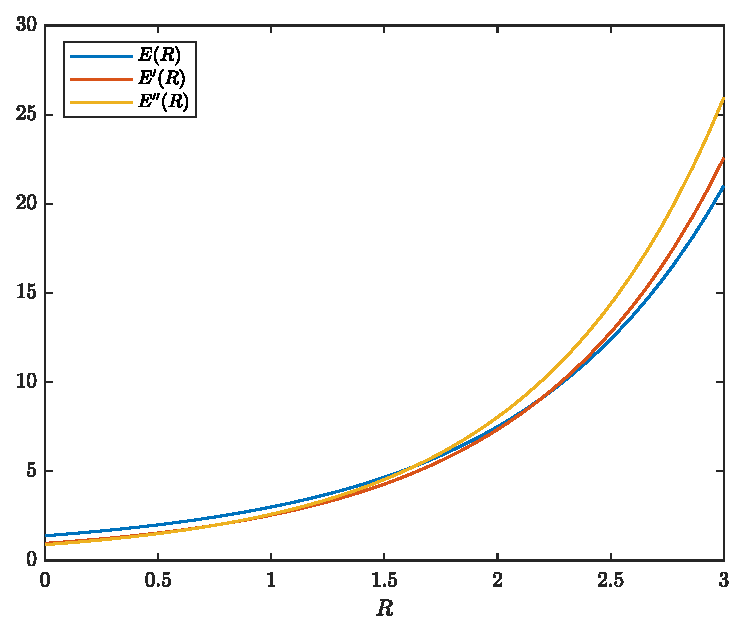
\includegraphics[width=0.7\linewidth]{img/energy_per_bit_1.eps}
	\caption{$E_b(R)$, $E'_b(R)$, $E''_b(R)$ for $R \leq \log\Big(\frac{g_2}{g_1}\Big)$ }
	\label{fig:funcex2}
\end{figure}

Note that these derivatives are pretty difficult to manage analytically. Fortunately, for low rates both derivatives are only a function of $R$ and multiplied by a constant positive factor $1/g_2^2$ which doesn't change the sign. Thus, we can see from Fig.~\ref{fig:funcex2} that at least for $R \leq \log\Big(\frac{g_2}{g_1}\Big)$, $E_b(R)$ is strictly increasing and convex. It can also be shown that the function is continuous on the splitting condition but showing anything analytically or even graphically on the second part of the function is not really easy since there is also the dependence from both $g_1$ and $g_2$. The only clear thing is that for $R \rightarrow \infty$ both derivatives are positive.

Now we want to compute the minimum energy-per-bit as $R \rightarrow 0$. We notice that for low values of $R$ we find ourself in the case where only one of the two channels is opened. Then to compute $\lim_{R \rightarrow 0} E_b(R)$ we proceed as follows.
%
\begin{equation}
	\lim_{R \rightarrow 0} E_b(R) =
		\lim_{R \rightarrow 0} \Big(\frac{2^{2R}-1}{g_2^2 R}\Big) = \lim_{R \rightarrow 0} \frac{ \frac{d(2^{2R}-1)}{dR}} {\frac{dg_2^2 R}{dR}}=\frac{2\ln{2}}{g_2^2}
\end{equation}

\numberwithin{equation}{section}
 %%%%%%%%
%\section*{Problem 3.14}
\mysection{3.14}{Problem 3.14}

\newcommand{\typical}{\ensuremath{\mathcal{T}_\varepsilon^{(n)}}}
\newcommand{\typicalLong}{\ensuremath{\mathcal{T}_\varepsilon^{(n)}(X^n,Y^n)}}

We decided to use the following coding/decoding scheme: the coder simply encodes the message $M$ into the codeword $X^n(M)$ like in the normal case seen in class. The decoder, instead, looks at all possible codewords $X^n(m) \; \forall m\in \mathcal{M}$, looks whether or not they are typical and creates $\mathcal{L}(Y^n) = \typicalLong$ if $|\typical| \leq 2^{nL}$ or $\mathcal{L}(Y^n)=\emptyset$ if $|\typical| > 2^{nL}$.

\numberwithin{equation}{subsection}
\subsection{Achievability}
Using the coder/decoder description given at the beginning of the section, the error probability can be written as
%
\begin{align}
\begin{split}
P_e^{(n)}=&E_\mathcal{C}[P_{e,\mathcal{C}}^n] = \Pr( M\notin \mathcal{L}(Y^n) |M=1 )\\
=& \Pr( \{(X^n(1),Y^n)\notin\typical| M=1\} \cup \{ |\typical|>2^{nL} \}|M=1)\\
\leq& \Pr((X^n(1),Y^n)\notin\typical|M=1) + \Pr(|\typical|>2^{nL}|M=1)\\
\triangleq& \Pr(\mathcal{E}_1) + \Pr(\mathcal{E}_2)
\end{split}
\end{align}

As seen in class, by the conditional typicality lemma $P(\mathcal{E}_1) \xrightarrow{n\rightarrow\infty}0$. All the effort, once again, will be focused on creating appropriate bounds for $\Pr(\mathcal{E}_2)$ as follows
%
\begin{align} \label{eq:3.14_E2}
\begin{split}
\Pr(\mathcal{E}_2) =& \Pr(|\typicalLong|>2^{nL}|M=1)\\
 \leq& \Pr(|\typicalLong| \geq 2^{nL}|M=1)\\
\leq& \frac{E \qty[\qty|\typicalLong| \,|M=1]}{2^{nL}}
\end{split}
\end{align}
%
where the last inequality follows from Markov's Inequality.

Now, we can bound the mean cardinality of the typicality set as follows:
%
\begin{align} \label{eq:3.14_expectation_bound}
\begin{split}
E \qty[\qty|\typicalLong| \,|M=1] =& E\qty[ \sum_{m=1}^{2^{nR}} \indicator((X^n(m),Y^n) \in \typical) |M=1 ]\\
=& \sum_{m=1}^{2^{nR}} E[\indicator((X^n(m),Y^n)\in \typical |M=1)]\\
=& \sum_{m=1}^{2^{nR}} \Pr((X^n(m),Y^n)\in \typical |M=1)\\
\leq& \Pr((X^n(1),Y^n)\in \typical |M=1)\\
& + \sum_{m=2}^{2^{nR}} \Pr((X^n(m),Y^n)\in \typical |M=1)\\
\stackrel{(a)}{\leq}& 1 + (2^{nR}-1)2^{-n(I(X;Y)-\delta(\varepsilon))}\\
\leq& 1 + 2^{-n(C-R - \delta(\varepsilon))}
\end{split}
\end{align}
%
where in $(a)$ we separated the probability of the first codeword to be typical with $Y^n$ since it has to be treated differently from the others (given the fact that actually $M=1$ was sent, so their probability of being jointly typical is higher than the rest) and we used the bound found in class for the rest of the codewords.

Now, joining Eqs.~\eqref{eq:3.14_expectation_bound},~\eqref{eq:3.14_E2} we obtain
%
\begin{equation}
P_e^{(n)} = \Pr(\mathcal{E}_1) + \Pr(\mathcal{E}_2) \leq \Pr(\mathcal{E}_1) +  2^{-nL} + 2^{-n(C+L-R - \delta(\varepsilon))}
\end{equation}
%
which tends to zero if $R<C+L$.

\subsection{Converse}
We will start showing the modified Fano's Inequality.

We are interested in the error probability defined as $P_e^{(n)} = \Pr(M \notin \mathcal{L}(Y^n))$. For this, similarly to the proof of Fano's Inequality seen in class, we define the random variable $\mathcal{E}$ such that $\mathcal{E}=0$ if $M \in \mathcal{L}$, $\mathcal{E}=1$ if $M \notin \mathcal{L}$. This implies that $E[\mathcal{E}] = P_e^{(n)}$ and $H(\mathcal{E}) = H(P_e^{(n)})$. Again, following the same procedure we obtain
%
\begin{equation}
H(M|\mathcal{L}) = H(\mathcal{E}|\mathcal{L})
+H(M|\mathcal{L},\mathcal{E})
-H(\mathcal{E}|M,\mathcal{L})
\end{equation}

Now, clearly $H(\mathcal{E}|M,\mathcal{L})=0$ since once we know the message $M$ and the list $\mathcal{L}$, we deterministically know the value of $\mathcal{E}$. Furthermore, $H(\mathcal{E}|\mathcal{L}) \leq H(\mathcal{E}) = H(P_e^{(n)})$ due to the conditional entropy property. Finally, we can write
%
\begin{equation}
H(M|\mathcal{E},\mathcal{L}) = P_e^{(n)} H(M|\mathcal{E}=1,\mathcal{L}) + (1-P_e^{(n)})H(M|\mathcal{E}=0,\mathcal{L})
\end{equation}
%
Now, if $\mathcal{E}=0$ it means that $M \in \mathcal{L}$, thus knowing both this and $\mathcal{L}$ means that $M$ could be any of the messages in the list, i.e. $H(M|\mathcal{L},\mathcal{E}=0) \leq \log_2|\mathcal{L}|$ (equal if the message is uniformly distributed). Similarly, if $M \notin \mathcal{L}$ it must be one of the other $|\mathcal{M}|-|\mathcal{L}|$ messages, i.e. $H(M|\mathcal{L},M\notin \mathcal{L}) \leq \log_2(|\mathcal{M}|-|\mathcal{L}|)$.

Bringing all together we get
%
\begin{align}
\begin{split}
H(M|\mathcal{L}) \leq & H(P_e^{(n)}) + P_e^{(n)}\log_2(|\mathcal{M}|-|\mathcal{L}|) + (1-P_e^{(n)})\log_2|\mathcal{L}|\\
=& H(P_e^{(n)}) + \log_2|\mathcal{L}| + P_e^{(n)}\log_2\qty(\frac{|\mathcal{M}|-|\mathcal{L}|}{|\mathcal{L}|})\\
=& H(P_e^{(n)}) + \log_2|\mathcal{L}| + P_e^{(n)}\log_2\qty(\frac{|\mathcal{M}|}{|\mathcal{L}|} - 1)\\
\leq& 1 + \log_2|\mathcal{L}| + P_e^{(n)}\log_2\frac{|\mathcal{M}|}{|\mathcal{L}|}
\end{split}
\end{align}

In our case we have $\mathcal{M}=2^{nR}$ and $1\leq |\mathcal{L}| \leq 2^{nL}$, thus we can upper bound $\log_2|\mathcal{L}| \leq nL$ and $\log_2(|\mathcal{M}|/|\mathcal{L}|) \leq nR$, thus yielding
%
\begin{equation}
H(M|\mathcal{L}) \leq 1+nL+P_e^{(n)} \, nR = nL + n\qty(\frac{1}{n} + P_e^{(n)} R) = nL + n\varepsilon_n
\end{equation}

Now the proof of the converse is exactly the same as the one seen in class, using this modified version of Fano's Inequality:
%
\begin{align}
\begin{split}
nR =& H(M)\\
=&  I(M;Y^n) + H(M|Y^n)\\
\stackrel{(a)}{\leq}& I(M;Y^n) + nL + n\varepsilon_n\\
=& \sum_{i=1}^n I(M;Y_i|Y^{i-1}) + nL+n\varepsilon_n\\
\stackrel{(b)}{\leq}& \sum_{i=1}^n I(M,Y^{i-1};Y_i) + nL+n\varepsilon_n\\
\stackrel{(c)}{=}& \sum_{i=1}^n I(M,X_i,Y^{i-1};Y_i) + nL+n\varepsilon_n\\
\stackrel{(d)}{=}& \sum_{i=1}^n I(X_i;Y_i) + nL+n\varepsilon_n\\
\leq& nC + nL+n\varepsilon_n
\end{split}
\end{align}
%
thus $R\leq C+L$ since $\varepsilon_n \xrightarrow{n\rightarrow\infty} 0$. In $(a)$ we used the fact that $\mathcal{L} \independent M |Y^n$ (or in Markov chain notation $M\rightarrow Y^n\rightarrow \mathcal{L}$), thus $H(M|Y^n)\leq H(M|\mathcal{L}) \leq nL + n\varepsilon_n$. In $(b)$ we used the conditioning rule $I(M,Y^{i-1};Y_i) = I(Y^{i-1};Y_i) + I(M;Y_i|Y^{i-1}) \geq I(M;Y_i|Y^{i-1})$. In $(c)$ we know that $X_i$ is a deterministic function of $M$ so it doesn't add or subtract any information. In $(d)$ we exploit the memoryless property of the channel and the conditional independence $Y_i \independent (M,Y^{i-1})|X_i$.

\numberwithin{equation}{section}

% !TEX root = C:\Users\Famiglia\Documents\GitHub\IT_homeworks\HW2\Solution.tex
\mysection{5.16}{Problem 5.16}
\renewcommand{\arraystretch}{2}
The k-receiver Gaussian Broadcast Channel is composed of k Gaussian BC's, one for each receiver. The output of the channel for the transmitted message $X$ at receiver 1 is $Y_1 = X+Z_1$ and at the $i-th$ receiver is $Y_i = X+Z_i$, where $Z_1,\tilde{Z}_2,...,\tilde{Z}_k$ are Gaussian noise components with powers $N_1,\tilde{N}_2,....,\tilde{N}_k$ respectively. We will assume that the notation is the same as the one used in chapter 5, i.e., the considered BC is degraded and receiver 1 is the strongest. \\
Let $m_i$ be the message destined to the $i$-th receiver, $i=1,2,...,k$.
\subsection{Achievability}
Achievability can be proved using superposition coding.
\subsubsection*{Codebook generation.}
 For each receiver $i$ fix a pmf $p(u_i)p(x|u_i)$. For each $i$, randomly and independently generate $2^{nR_i}$ sequences $u^n_i(m_i)$, $m_i\in [1:2^{nR_i}]$, $U_i\sim \mathcal{N}(0, \alpha_i P)$, with $\alpha_1 = 1-\sum_{h=2}^k \alpha_h$.
According to the superposition coding, to transmit $m_1,m_2,...,m_k$ the transmitter sends
\begin{equation}
X = U_1+ U_2+...+U_k = \sum_{i=1}^k U_i
\end{equation}
We will use the word "message" to denote both the message $m$ and its encoded version $u$ since they play the same role in this dimostration.
\subsubsection*{Encoding}
To send $(m_1,m_2,....,m_k)$ transmit $x^n(m_1,m_2, ...,m_k)$.
\subsubsection*{Decoding}
\begin{itemize}
\item \textbf{@ receiver k} Receiver $k$ receives
\begin{equation}
Y_k = Y_{k-1}+\tilde{Z}_k = .. = U_1 + U_2 + ... +U_k + Z_k
\end{equation}
Applying the \underline{superposition decoding}, receiver $k$ treats $\sum_{h=1}^{k-1} U_h$ as noise, together with $Z_k$. Accordingly, and applying the knowledge of the point-to-point Gaussian channel, we know that the probability of error goes to zero if
\begin{equation}
  R_k<C\left(\frac{S}{N}\right) = C\left(\frac{\alpha_k P}{\left(\sum_{h=1}^{k-1}\alpha_h \right)P + N_k}\right) = C\left(\frac{\alpha_k P}{\left(1-\alpha_k\right)P + N_k}\right)
  \label{eq:k_cond_superpos}
\end{equation}
\item \textbf{@ receiver i} Receiver $i$, $i\neq 1,k$, receives
\begin{equation}
Y_i = Y_{i-1}+\tilde{Z}_i = .. = U_1 + U_2 + ... +U_k + Z_i
\end{equation}
First, $U_k$ is retrieved, using the same procedure as in the previous case.
As before, the probability of error goes to zero if
\begin{equation}
  R_k<C\left(\frac{S}{N}\right) = C\left(\frac{\alpha_k P}{\left(\sum_{h=1}^{k-1}\alpha_h \right)P + N_i}\right) = C\left(\frac{\alpha_k P}{\left(1-\alpha_k\right)P + N_i}\right)
  \label{eq:i_cond_superpos}
\end{equation}
Notice that the only difference with the previous case is the noise term at the denominator. Since $N_k>N_i\ \forall i\leq k$,
\begin{equation}
  C\left(\frac{\alpha_k P}{\left(1-\alpha_k\right)P + N_k}\right)<C\left(\frac{\alpha_k P}{\left(1-\alpha_k\right)P + N_i}\right)
\end{equation}
and therefore the condition in \ref{eq:k_cond_superpos} implies the condition in \ref{eq:i_cond_superpos}.\\
Knowing $U_k$, we can substract it from the received signal:
\begin{equation}
Y_i - U_k = U_1 + U_2 + ... +U_{k-1} + Z_i
\end{equation}
We can now repeat the exact same procedure to obtain all the messages up to $U_i$. At each step $l$, $i\leq l \leq k$, a new condition analogous to \ref{eq:i_cond_superpos} in the form of:
\begin{equation}
  R_l< C\left(\frac{\alpha_l P}{\left(\sum_{h=1}^{l-1}\alpha_h P+N_i\right)}\right)
\end{equation}
 must be satisfied to guarantee the correct decoding of $U_l$.
\item \textbf{@ receiver 1} proceeding iteratively, it is possible to decode all the messages up to message $u_1$. The last condition is
\begin{equation}
  R_1<C\left(\frac{\alpha_1 P}{N_1}\right)
\end{equation}
\end{itemize}
The set of conditions obtained during the decoding is summarized in table \ref{tab:conditions}.
\begin{table}[h!]
  \centering
  \begin{tabular}{c|c|c|c|c}
      Receiver & $R_k$ & $R_{k-1}$ &.. & $R_1$ \\
      \hline
      $k$ & $R_k<C\left(\frac{\alpha_k P}{\left(1-\alpha_k\right)P + N_k}\right)$ & - & .. & -\\
      $k-1$ & $R_k<C\left(\frac{\alpha_{k} P}{\left(1-\alpha_k\right)P + N_{k-1}}\right)$ & $R_{k-1}<C\left(\frac{\alpha_{k-1} P}{\left(1-\alpha_k-\alpha_{k-1}\right)P + N_{k-1}}\right)$ & .. & -\\
      . & . & . & . & . \\
      . & . & . & . & . \\
      . & . & . & . & . \\
      2 & $R_k<C\left(\frac{\alpha_{k} P}{\left(1-\alpha_k\right)P + N_{2}}\right)$ & $R_{k-1}<C\left(\frac{\alpha_{k-1} P}{\left(1-\alpha_k-\alpha_{k-1}\right)P + N_{2}}\right)$ & .. & - \\
      1 & $R_k<C\left(\frac{\alpha_{k} P}{\left(1-\alpha_k\right)P + N_{1}}\right)$ & $R_{k-1}<C\left(\frac{\alpha_{k-1} P}{\left(1-\alpha_k-\alpha_{k-1}\right)P + N_{1}}\right)$ & .. & $R_{1}<C\left(\frac{\alpha_{1} P}{N_{1}}\right)$\\
  \end{tabular}
  \caption{Conditions on the rate of each channel, at each receiver.}
  \label{tab:conditions}
\end{table}
As noticed before, the conditions can be simplified as in table \ref{tab:conditions_fin} considering that $N_k\geq N_{k-1}\geq ... \geq N_1$: the rate for channel $i$ is :
\begin{equation}
  R_i < C\left(\frac{\alpha_i P}{\sum_{h<i}\alpha_h P +N_i}\right)
\end{equation}
\begin{table}[h!]
\centering
  \begin{tabular}{c|c|c|c}
      $R_k$ & $R_{k-1}$ &.. & $R_1$ \\
      \hline
      $R_k<C\left(\frac{\alpha_k P}{\left(1-\alpha_k\right)P + N_k}\right)$ & $R_{k-1}<C\left(\frac{\alpha_{k-1} P}{\left(1-\alpha_k-\alpha_{k-1}\right)P + N_{k-1}}\right)$ & .. & $R_{1}<C\left(\frac{\alpha_{1} P}{N_{1}}\right)$\\
  \end{tabular}
  \caption{Summary of the conditions on the rate of each channel.}
  \label{tab:conditions_fin}
\end{table}
\subsection{Converse}
To prove the converse, we need to prove that for every code with rates $R_1, R_2, .., R_k$ there exists a sequence $\alpha_1, \alpha_2, ... , \alpha_k$, $\sum_{h=1}^k\alpha_k = 1$, such that
\begin{align}
  \centering
  \begin{split}
    & R_k<C\left(\frac{\alpha_k P}{\left(1-\alpha_k\right)P + N_k}\right),\\
    & R_i<C\left(\frac{\alpha_i P}{\sum_{h<i}\alpha_h P +N_i}\right),\text{ for } i = 2,..,k-1.\\
    & R_{1}<C\left(\frac{\alpha_{1} P}{N_{1}}\right),\\
  \end{split}
\end{align}

We will start from receiver $k$. Using Fano's inequality the converse condition can be written as
\begin{equation}
  nR_k\leq I(M_k;Y^n_k)
\end{equation}
Therefore to prove the converse we can just prove that
\begin{align}
  \begin{split}
    I(M_k;Y^n_k)\leq nC\left(\frac{\alpha_k P}{\left(1-\alpha_k\right)P + N_k}\right) = \frac{n}{2}\log\left(1+\frac{\alpha_k P}{\left(1-\alpha_k\right)P + N_k}\right)=\\
    =\frac{n}{2}\log\left(\frac{P+N_k}{\left(1-\alpha_k\right)P + N_k}\right)
  \end{split}
\end{align}
Let us consider the first term of the previous equation. Applying the properties of the mutual information, we get that
\begin{align}
  \begin{split}
    I(M_k;Y_k^n) = h(Y_k^n) - h(Y_k^n|M_k)
    \leq \frac{n}{2}\log(2\pi e (P+N_k))- h(Y_k^n|M_k)
    \label{eq:I_M_K}
  \end{split}
\end{align}
Consider the last term of equation \ref{eq:I_M_K}:
\begin{align}
  \begin{cases}
  h(Y_k^n|M_k)\geq h(Y_k^n|X^n,M_k) = h(Z^n_k) = \frac{n}{2}\log\left(2\pi e N_k\right) \\
  h(Y_k^n|M_k)\leq h(Y_k^n)\leq \frac{n}{2} \log(2\pi e (P+N_k))\\
  \end{cases}
  \\
  \implies \frac{n}{2}\log\left(2\pi e N_k\right)\leq h(Y_k^n|M_k) \leq \frac{n}{2} \log(2\pi e (P+N_k))
\end{align}
Therefore, there must exist a $\alpha_k \in [0,1]$ such that
\begin{equation}
  h(Y_k^n|M_k) = \frac{n}{2}\log(2\pi e ((1-\alpha_k) P+N_k))
  \label{eq:Y_kM_k}
\end{equation}
Substituing \ref{eq:Y_kM_k} in \ref{eq:I_M_K}, we obtain
\begin{align}
  \begin{split}
    I(M_k;Y_k^n) \leq \frac{n}{2}\log(2\pi e (P+N_k))- h(Y_k^n|M_k) =\\ =\frac{n}{2}\log(2\pi e (P+N_k))-\frac{n}{2}\log(2\pi e ((1-\alpha_k) P+N_k))\\
    = \frac{n}{2}\log(\frac{P+N_k}{(1-\alpha_k)P+N_k})
  \end{split}
  \label{eq:I_M_K}
\end{align}
and this demonstrates the converse for rate $R_k$.\\

A similar procedure can be applied to receiver $k-1$. The converse can be proved if we demonstrate that
\begin{align}
  \begin{split}
    nR_{k-1}\leq I(M_{k-1};Y_{k-1})\leq nC\left(\frac{\alpha_{k-1} P}{\left(1-\alpha_k-\alpha_{k-1}\right)P + N_{k-1}}\right) = \\
    = \frac{n}{2}\log\left(1+\frac{\alpha_{k-1} P}{\left(1-\alpha_k-\alpha_{k-1}\right)P + N_{k-1}}\right)\\
    = \frac{n}{2}\log\left(\frac{(1-\alpha_{k})P+N_{k-1} }{\left(1-\alpha_k-\alpha_{k-1}\right)P + N_{k-1}}\right)\\
    = \frac{n}{2}\log\left((1-\alpha_{k})P+N_{k-1}\right)-\frac{n}{2}\log\left(\left(1-\alpha_k-\alpha_{k-1}\right)P + N_{k-1}\right)
  \end{split}
\end{align}
First, we notice that for the properties of the mutual information and the independency of $M_k$, $M_{k-1}$:
\begin{equation}
  I(M_{k-1};Y^n_{k-1})\leq I(M_{k-1};Y^n_{k-1}|M_k)
\end{equation}
so for the converse we can just prove that
\begin{equation}
  I(M_{k-1};Y^n_{k-1}|M_k)\leq \frac{n}{2}\log\left((1-\alpha_{k})P+N_{k-1}\right)-\frac{n}{2}\log\left(\left(1-\alpha_k-\alpha_{k-1}\right)P + N_{k-1}\right)
  \label{eq:I_M-1_K-1}
\end{equation}
Again, as in \ref{eq:I_M_K}, we can express
\begin{equation}
  I(M_{k-1};Y^n_{k-1}|M_k) = h(Y_{k-1}^n|M_{k}) - h(Y_{k-1}^n|M_k,M_{k-1}).
  \label{eq:I_M_K-1_I_K-1|Mk}
\end{equation}
\begin{itemize}
  \item $\mathbf{h(Y_{k-1}^n|M_{k})}$. First, consider $h(Y_k^n|M_k)$. Recalling the definition of the degraded Gaussian BC, we know that
  \begin{equation}
      Y^n_k = Y^n_{k-1}+\tilde{Z}^n_k
  \end{equation}
  and applying the Entropy Power Inequality (EPI):
  \begin{align}
    \begin{split}
      2^{2h(Y^n_k|M_k)/n}\geq 2^{2h(Y^n_{k-1}|M_k)/n}+2^{2h(\tilde{Z}^n_{k}|M_k)/n}
    \end{split}
    \label{eq:EPI}
  \end{align}
  Since $\tilde{Z}^n_k$ and $M_k$ are independent, and $\tilde{Z}^n_k$ is distributed as $\mathcal{N}(0,\tilde{N}_k)$
  \begin{align}
    \begin{split}
      h(\tilde{Z}^n_{k}|M_k) = h(\tilde{Z}^n_{k}) = \frac{n}{2}\log\left(2\pi e \tilde{N}_k\right).
    \end{split}
  \end{align}
  Using this result in the \ref{eq:EPI}, and taking the logarithm in both sides,
  \begin{align}
    \begin{split}
      2h(Y^n_k|M_k)/n\geq \log\left(2^{2h(Y^n_{k-1}|M_k)/n}+2^{\log\left(2\pi e \tilde{N}_k\right)}\right) \\
      = \log\left(2^{2h(Y^n_{k-1}|M_k)/n}+2\pi e \tilde{N}_k\right)\\
      \implies h(Y^n_k|M_k)\geq \frac{n}{2}\log\left(2^{2h(Y^n_{k-1}|M_k)/n}+2\pi e \tilde{N}_k\right)
    \end{split}
  \end{align}
  Now, we go back to decoder $k$ and use again the result in \ref{eq:Y_kM_k}, from the above equation we obtain that
  \begin{equation}
    h(Y_k^n|M_k) = \frac{n}{2}\log(2\pi e ((1-\alpha_k) P+N_k))\geq \frac{n}{2}\log\left(2^{2h(Y^n_{k-1}|M_k)/n}+2\pi e \tilde{N}_k\right)
  \end{equation}
  Since the logarithm is monotonically increasing, we can move the relation to the arguments:
  \begin{align}
    \begin{split}
      2\pi e ((1-\alpha_k) P+N_k))\geq (2^{2h(Y^n_{k-1}|M_k)/n}+2\pi e \tilde{N}_k\\
      \implies
      2\pi e ((1-\alpha_k) P+N_k-\tilde{N}_k)\geq 2^{2h(Y^n_{k-1}|M_k)/n}\\
      \implies
      \log(2\pi e ((1-\alpha_k) P+N_k-\tilde{N}_k))\geq 2h(Y^n_{k-1}|M_k)/n\\
      \implies
      \frac{n}{2}\log(2\pi e ((1-\alpha_k) P+N_k-\tilde{N}_k))\geq h(Y^n_{k-1}|M_k)
    \end{split}
    \label{eq:Yk-1_Mk}
  \end{align}
  For the structure of the degraded Gaussian BC, $N_k-\tilde{N}_k=N_{k-1}$ and \ref{eq:Yk-1_Mk} becomes
  \begin{align}
    \frac{n}{2}\log(2\pi e ((1-\alpha_k) P+N_{k-1}))\geq h(Y^n_{k-1}|M_k)
    \label{eq:Yk-1|Mk}
  \end{align}
  that is the first term in \ref{eq:I_M-1_K-1}, so:
  \begin{align}
    \begin{split}
        I(M_{k-1};Y^n_{k-1}|M_k) = h(Y_{k-1}^n|M_{k}) - h(Y_{k-1}^n|M_k,M_{k-1})\leq\\
        \leq \frac{n}{2}\log(2\pi e ((1-\alpha_k) P+N_{k-1})) - h(Y_{k-1}^n|M_k,M_{k-1})
    \end{split}
    \label{eq:final_1}
  \end{align}
  \item $\mathbf{h(Y_{k-1}^n|M_k,M_{k-1})}$. Consider now the second term in \ref{eq:I_M_K-1_I_K-1|Mk}. We can apply the same reasoning as in \ref{eq:Y_kM_k} and set the sequence of disequations:
  \begin{align}
    \begin{cases}
      h(Y_{k-1}|M_{k-1},M_{k})\geq h(Y_{k-1}|M_{k-1},M_{k},X) =h(Z_{k-1}) = \frac{n}{2}\log(2\pi e N_{k-1}) \\
      h(Y_{k-1}|M_{k-1},M_{k})\leq h(Y_{k-1}|M_{k})\overset{(\ref{eq:Yk-1|Mk})}{\leq} \frac{n}{2}\log(2\pi e ((1-\alpha_k) P+N_{k-1}))
    \end{cases}
  \end{align}
  from which
  \begin{equation}
    \frac{n}{2}\log(2\pi e N_{k-1})\leq h(Y_{k-1}|M_{k-1},M_{k})\leq \frac{n}{2}\log(2\pi e ((1-\alpha_k) P+N_{k-1}))
  \end{equation}
  and therefore there must exist $\alpha_{k-1}$ such that
  \begin{equation}
    h(Y_{k-1}|M_{k-1},M_{k}) = \frac{n}{2}\log(2\pi e ((1-\alpha_k-\alpha_{k-1}) P+N_{k-1})).
    \label{eq:final_2}
  \end{equation}
  The parameter $\alpha_{k-1}$ is positive and must vary in such a way so that
  \begin{equation*}
    0\leq(1-\alpha_k-\alpha_{k-1})\leq 1
    \implies 0\leq\alpha_{k-1}\leq 1-\alpha_k
  \end{equation*}
\end{itemize}
Combining the previous points:
\begin{align}
  \begin{split}
    I(M_{k-1};Y^n_{k-1}|M_k) = h(Y_{k-1}^n|M_{k}) - h(Y_{k-1}^n|M_k,M_{k-1})\leq\\
    \overset{(\ref{eq:final_1})}{\leq} \frac{n}{2}\log(2\pi e ((1-\alpha_k) P+N_{k-1})) - h(Y_{k-1}^n|M_k,M_{k-1}) =\\
    \overset{(\ref{eq:final_2})}{=}\frac{n}{2}\log(2\pi e ((1-\alpha_k) P+N_{k-1}))-\frac{n}{2}\log(2\pi e ((1-\alpha_k-\alpha_{k-1}) P+N_{k-1}))=\\
    = \frac{n}{2}\log\left(\frac{((1-\alpha_k) P+N_{k-1}}{(1-\alpha_k-\alpha_{k-1}) P+N_{k-1}}\right)
  \end{split}
  \label{eq:final_k-1}
\end{align}
Now the procedure can be iterated for every $1\leq i\leq k-1$ in the same way. At every step $i$, the condition on $\alpha_i$ is
\begin{equation}
  0\leq \alpha_i \leq 1-\sum_{h>i}\alpha_h
\end{equation}
up to the first receiver, where $\alpha_1 = 1-\sum_{h\neq 1}\alpha_h$ so that the power constrain is also satisfied:
\begin{equation}
\sum_{h = 1}^k \alpha_h = 1.
\end{equation}

% and considering the fact that $M_i$ is independent of any other $M_h$ with $h\leq i$, for the properties of the mutual information
% \begin{equation}
%   nR_i\leq I(M_i;Y^n_i)\leq I(M_i;Y^n_i|M_h).
% \end{equation}
% Therefore to prove the converse we can just prove that
% \begin{equation}
%   I(M_i;Y^n_i|M_h)\leq nC\left(\frac{\alpha_i P}{\sum_{h<i}\alpha_h P +N_i}\right).
% \end{equation}
% Consider $I(M_i;Y_i^n|M_{h<i})$ where $M_{h<i} = M_1,...,M_{i-1}$. Applying the properties of the mutual information, we get that
% \begin{align}
%   \begin{split}
%     I(M_i;Y_i^n|M_{h<i}) = h(Y_i^n|M_{h<i}) - h(Y_i^n|M_i,M_{h<i}) = h(Y_i^n|M_{h<i}) - h(Y_i^n|M_{h\leq i})\\
%     \leq \frac{n}{2}\log(2\pi e (P+N_i))- h(Y_i^n|M_{h\leq i})
%     \label{eq:I_M_Y}
%   \end{split}
% \end{align}
% Let us analyse the first term:
% \begin{align*}
%   \frac{n}{2}\log(2\pi e N_i) = h(Y^n_i|M_h) \leq h(Y^n_i|M_{h\leq i})\leq \frac{n}{2}\log(2\pi e (P+N_i)).
% \end{align*}
% Then, there exists $\alpha_i \in [0,1]$ such that
% \begin{equation}
%   h(Y_i^n|M_{h\leq i}) = \frac{n}{2} \log(2\pi e (\alpha_i P+N_i)).
%   \label{eq:h_Y}
% \end{equation}
% Applying \ref{eq:h_Y} to \ref{eq:I_M_Y}, we obtain
% \begin{equation}
%   I(M;Y_i^n|M_{h<i})\leq \frac{n}{2}\log\left(\frac{P+N_i}{\alpha_i P + N_i}\right)
% \end{equation}


\end{document}
